%!TeX program = xelatex
%!TeX options = -shell-escape
% this template mostly comes from Trinkle23897
% his github repo is https://github.com/Trinkle23897/THU-Beamer-Theme
% thanks a lot Trinkle!
% two color theme fdu_red and fdu_blue, choose your preference main document and switch in the menu
% github repo https://github.com/milanmarks/FDU-Beamer-Theme

%%%%%%%%%%%%%%%%%%%%%%%%%%%%%%%%%%%%%%%%%%
% 导言区 
%%%%%%%%%%%%%%%%%%%%%%%%%%%%%%%%%%%%%%%%%%
\documentclass{beamer}
\usepackage{ctex, hyperref}
\usepackage[T1]{fontenc}
% other packages
\usepackage{latexsym,amsmath,xcolor,multicol,booktabs,calligra}
\usepackage{graphicx,pstricks,listings,stackengine}
\usepackage{tabularx}
\usepackage{minted}
\usemintedstyle{colorful} % 可以选择不同的高亮风格，如 monokai, friendly, colorful 等
\usepackage{tikz}
\usetikzlibrary{shapes.geometric, arrows, positioning}

% 字体
%\setCJKmainfont{FandolSong-Regular}[Script=Default,Language=Default]
%\setmonofont{DejaVu Sans Mono}

% bibtex setting
% 引入 biblatex 宏包
% style=alphabetic 对应你原来的 alpha 样式
% maxnames=3 表示最多显示3个作者，超出的自动变 et al.
%\usepackage[backend=biber, style=alphabetic, maxnames=3]{biblatex}
% 指定你的 .bib 文件
%\addbibresource{ref.bib}

%%%%%%%%%%%%%%%%%%%%%%%%%%%%%%%%%%%%%%%%%%%%%
% 个人信息区
%%%%%%%%%%%%%%%%%%%%%%%%%%%%%%%%%%%%%%%%%%%%%
\author{周律邦}
\title{"算丰杯"医疗AI Skill开发大赛}
\subtitle{SMA 高值特药理赔合规审核 Skill}
\institute{中国医学科学院 \& 北京协和医学院}
\date{5 July 2026}
\usepackage{RenminUniv}

% defs
\def\cmd#1{\texttt{\color{green}\footnotesize $\backslash$#1}}
\def\env#1{\texttt{\color{blue}\footnotesize #1}}
\definecolor{deepblue}{rgb}{0,0,0.5}
\definecolor{deepgreen}{rgb}{0.6,0,0}
\definecolor{lightgreen}{rgb}{0,0.5,0}
\definecolor{halfgray}{gray}{0.55}

\newcommand{\tagbad}{\textcolor{red!70!black}{高风险}}

\lstset{
    basicstyle=\ttfamily\small,
    keywordstyle=\bfseries\color{deepblue},
    emphstyle=\ttfamily\color{deepgreen},    % Custom highlighting style
    stringstyle=\color{lightgreen},
    numbers=left,
    numberstyle=\small\color{halfgray},
    rulesepcolor=\color{red!20!green!20!blue!20},
    frame=shadowbox,
}


\begin{document}

\kaishu
\begin{frame}
    \titlepage
    \begin{figure}[htpb]
        \begin{center}
            
\includegraphics[width=0.15\linewidth]{pic/pumc-logo.png}
        \end{center}
    \end{figure}
\end{frame}

\begin{frame}[fragile]{目录}
\tableofcontents[sectionstyle=show,subsectionstyle=show/shaded/hide,subsubsectionstyle=show/shaded/hide]
\end{frame}

\section{场景描述}

\begin{frame}[fragile]{业务场景}
  \begin{itemize}
    \item 罕见病高值药的关键业务环节，不是简单投保核保，而是理赔、报销、特药责任审核。
    \item SMA治疗涉及高值药、遗传学证据、专科处方、用药记录和医保/商保支付条件。
    \item V1聚焦两个MVP药物：诺西那生钠和利司扑兰。
    \item Skill目标是完成材料初筛和风险提示，辅助人工复核。
  \end{itemize}
\end{frame}

\begin{frame}[fragile]{为什么选择SMA}
  \begin{tabularx}{\textwidth}{>{\bfseries}l X}
    \toprule
    维度 & 说明 \\
    \midrule
    差异化 & 相比常见肿瘤核保，SMA高值药更贴近罕见病特药支付审核。 \\
    可结构化 & 诊断、基因检测、药物、给药方式、处方和支付材料均可拆成明确字段。 \\
    可验证 & 可以构造完整病历材料包，验证Skill是否能抽取字段并命中规则。 \\
    可扩展 & 后续可扩展到DMD（杜氏肌营养不良症）、血友病、戈谢病等高值药场景。 \\
    \bottomrule
  \end{tabularx}
\end{frame}

\begin{frame}[fragile]{V1边界}
  \begin{itemize}
    \item 不做最终赔付决定。
    \item 不提供治疗建议、换药建议或预后判断。
    \item 不实时判断最新医保目录和地方政策。
    \item 只输出资料完整性、适应证匹配、支付条件匹配、风险提示和补充材料。
    \item 借鉴平台提供的“智能核保示例 SKILL” 风格进行制作，形成 V1 。
  \end{itemize}
\end{frame}

\section{需求分析}
\begin{frame}[fragile]{审核对象}
\setlength{\tabcolsep}{8pt}
\renewcommand{\tabularxcolumn}[1]{m{#1}}
\begin{tabularx}{\textwidth}{
  >{\hsize=0.6\hsize}X
  >{\hsize=0.7\hsize}X
  >{\hsize=0.8\hsize}X
  >{\hsize=1.9\hsize}X
}
    \toprule
    药物 & 商品名 & 给药方式 & V1审核重点 \\
    \midrule
    诺西那生钠 & Spinraza & 鞘内注射 & 5q SMA、SMN1证据、鞘内注射/腰穿记录、负荷/维持给药、专科处方。 \\
    利司扑兰 & Evrysdi & 口服 & 5q SMA、SMN1证据、年龄/体重、剂量依据、连续领药/用药记录、专科处方。 \\
    \bottomrule
  \end{tabularx}
\end{frame}

\begin{frame}[fragile]{输入材料需求}
  \begin{columns}[T,onlytextwidth]
    \begin{column}{0.48\textwidth}
      \begin{block}{医学材料}
        \begin{itemize}
          \item 神经肌肉专科病历
          \item 5q SMA诊断证明
          \item SMN1/SMN2基因检测
          \item SMA分型或起病年龄
          \item 功能评分或运动功能描述
        \end{itemize}
      \end{block}
    \end{column}
    \begin{column}{0.48\textwidth}
      \begin{block}{支付材料}
        \begin{itemize}
          \item 药物处方和医嘱
          \item 用药记录、发票、费用清单
          \item 医保结算单
          \item 商保条款或特药清单
          \item 指定医院/药房和授权备案
        \end{itemize}
      \end{block}
    \end{column}
  \end{columns}
\end{frame}

\begin{frame}[fragile]{执行流程}
  \begin{enumerate}
    \item Step 0：提示用户提交病历、基因检测、处方、发票和条款。
    \item Step 1：按10项Checklist标注已获得、不明确、缺失。
    \item Step 2：先查资料完整性，再查适应证，再查支付条件，最后筛高风险。
    \item Step 3：按固定模板输出案件摘要、结论、依据、风险和补充材料。
  \end{enumerate}
  \vspace{0.5em}
  \begin{block}{控制点}
    缺失字段不假设；一轮最多追问3个问题；不承诺赔付。
  \end{block}
\end{frame}

\begin{frame}[fragile]{Checklist字段}
  \begin{tabularx}{\textwidth}{c X c X}
    \toprule
    序号 & 字段 & 序号 & 字段 \\
    \midrule
    1 & 年龄、性别、体重、申请日期 & 6 & 处方机构、科室、医生 \\
    2 & SMA诊断，是否5q SMA & 7 & 鞘内注射或口服领药记录 \\
    3 & SMN1/SMN2基因检测 & 8 & 既往SMA治疗史 \\
    4 & SMA分型或运动功能状态 & 9 & 发票、费用清单、医保结算单 \\
    5 & 药物、剂量、给药方式 & 10 & 条款、清单、授权备案材料 \\
    \bottomrule
  \end{tabularx}
\end{frame}

\section{验证病例}
\subsection{病例验证设计}
\begin{frame}[fragile]{验证设计}
  \begin{itemize}
    \item 每个病例采用平台示例式“完整病历输入格式”。
    \item 验证时输入较为格式化的病例正文。
    \item 输出后对照预期结果，检查字段抽取、规则命中、结论稳定性和合规边界。
    \item 采用平台提供的 大模型 API ，如 DEEPSEEK-V4-Pro。
  \end{itemize}
  \vspace{0.5em}
  \begin{block}{合格标准}
    能稳定输出五大模块，并准确识别关键风险点。
  \end{block}
\end{frame}

\begin{frame}[fragile]{五个验证病例}
  \begin{tabularx}{\textwidth}{l X X}
    \toprule
    病例 & 输入特征 & 预期重点 \\
    \midrule
    1 & 5q SMA II型，诺西那生钠，鞘内记录齐全 & 可进入人工复核 \\
    2 & 疑似SMA，基因报告未出，申请利司扑兰 & 关键缺失，信息不足 \\
    3 & 诺西那生钠发票，但记录为每日口服 & 给药方式和材料冲突 \\
    4 & 利司扑兰诊断证据完整，但缺少支付材料 & 适应证符合，支付需复核 \\
    5 & 投保前确诊，基因治疗后又申请诺西那生钠 & 既往症、等待期、序贯治疗高风险 \\
    \bottomrule
  \end{tabularx}
\end{frame}

\subsection{病例材料与简介}
\begin{frame}[fragile]{病例1：材料较完整}
  \begin{block}{输入摘要}
    3岁女童，5q SMA II型；SMN1第7、8外显子纯合缺失，SMN2 3拷贝；申请诺西那生钠；已有儿童神经专科处方、鞘内注射记录、发票和费用清单。\cite{RN65}
  \end{block}
  \begin{tabularx}{\textwidth}{l X}
    \toprule
    模块 & 预期输出 \\
    \midrule
    资料完整性 & 材料链基本完整。 \\
    适应证匹配 & 诊断、遗传学证据和给药方式匹配。 \\
    支付条件匹配 & 需核验特药清单有效日期、指定医院和授权备案。 \\
    综合结论 & 可进入人工理赔复核。 \\
    \bottomrule
  \end{tabularx}
\end{frame}

\begin{frame}[fragile]{病例2：疑似SMA，缺少遗传学证据}
  \begin{block}{输入摘要}
    8个月男婴，临床表现为抬头不稳、翻身困难、肌张力低，门诊病历仅写“疑似SMA”；家属称已送检SMN1/SMN2基因检测但报告未出；申请利司扑兰，尚未开始用药，仅提交处方照片，未提供医保目录或商保条款。\cite{iwayama2025delayed}
  \end{block}
  
  \vspace{0.5em} % 可选：稍微增加一点块和表格之间的间距
  
  % 在这里加入字号缩小命令，比如 \small, \footnotesize, \scriptsize 或 \tiny
  \footnotesize 
  \begin{tabularx}{\textwidth}{l X}
    \toprule
    模块 & 预期输出 \\
    \midrule
    资料完整性 & 关键缺失：缺少正式基因检测报告、正式诊断证明、发票和用药记录。 \\
    适应证匹配 & 信息不足：仅有疑似SMA，尚不能确认5q SMA及SMN1遗传学证据。 \\
    支付条件匹配 & 无法判断或需人工复核：未提供医保目录、商保条款或特药清单。 \\
    高风险筛查 & 命中R1疑似诊断无基因证据，R2非5q SMA或证据不足。 \\
    综合结论 & 暂不具备审核条件，需补充材料后再进入理赔复核。 \\
    \bottomrule
  \end{tabularx}
\end{frame}

\begin{frame}[fragile]{病例3：材料冲突}
  \begin{block}{输入摘要}
    5岁女童，5q SMA III型；申请表和发票为诺西那生钠，但处方照片疑似利司扑兰，用药记录写每日口服一次，未提供鞘内注射记录。
  \end{block}
  \begin{tabularx}{\textwidth}{l X}
    \toprule
    模块 & 预期输出 \\
    \midrule
    资料完整性 & 关键缺失。 \\
    适应证匹配 & 信息不足。 \\
    高风险筛查 & 命中R3诺西那生钠缺少鞘内记录，R5材料冲突。 \\
    综合结论 & 高风险需人工复核。 \\
    \bottomrule
  \end{tabularx}
\end{frame}

\begin{frame}[fragile]{病例4：适应证符合但支付依据缺失}
  \begin{block}{输入摘要}
    16岁男性，5q SMA III型；SMN1第7外显子纯合缺失，SMN2 4拷贝；申请利司扑兰，已提供神经内科处方、发票、连续领药记录和随访病历，但缺少医保结算单、商保特药责任条款、有效特药清单、指定药房证明和事前授权材料。\cite{saito2025safety}
  \end{block}
  \vspace{0.5em} % 可选：稍微增加一点块和表格之间的间距
  
  % 在这里加入字号缩小命令，比如 \small, \footnotesize, \scriptsize 或 \tiny
  \footnotesize 
  \begin{tabularx}{\textwidth}{l X}
    \toprule
    模块 & 预期输出 \\
    \midrule
    资料完整性 & 关键缺失：医学材料较完整，但支付依据和流程材料缺失。 \\
    适应证匹配 & 符合：诊断、SMN1证据、申请药物和口服用药场景匹配。 \\
    支付条件匹配 & 需人工复核：无法确认特药清单、指定药房、医保先行支付及授权备案要求。 \\
    高风险筛查 & 命中R8指定医院/药房、事前授权或医保先行支付流程不明。 \\
    综合结论 & 可进入人工复核，但不能直接判定支付条件符合。 \\
    \bottomrule
  \end{tabularx}
\end{frame}

\begin{frame}[fragile]{病例5：既往症与序贯治疗风险}
  \begin{block}{输入摘要}
    2岁女童，2025年6月确诊5q SMA I型；2025年12月基因治疗，2026年2月利司扑兰，2026年4月申请诺西那生钠；商业保险2026年1月15日生效，等待期90天。\cite{okubo2026outcomes}
  \end{block}
  \begin{itemize}
    \item 命中R6：多药序贯或联合治疗依据不足。
    \item 命中R7：既往症、等待期、责任免除风险。
    \item 可能命中R3：缺少正式鞘内注射记录。
    \item 综合结论：\tagbad，高风险需人工复核。
  \end{itemize}
\end{frame}

\section{V1：病例测试与展示}

\subsection{V1 完成部分}
\begin{frame}[fragile]{V1 完成部分}
  \begin{tabularx}{\textwidth}{l X}
    \toprule
    交付物 & 状态 \\
    \midrule
    主Skill文件 & 已完成平台风格应用于SMA药物核保的 SKILL。 \\
    完整病历测试集 & 已完成5个病例的测试，病例来自于相关论文。 \\
    预期输出文件 & 已完成，用于人工对照。 \\
    \bottomrule
  \end{tabularx}
\end{frame}

\subsection{病例1 结果与对比}
\begin{frame}[fragile]{病例1 实操与结果输出}
    \centering
    % 图片区域
    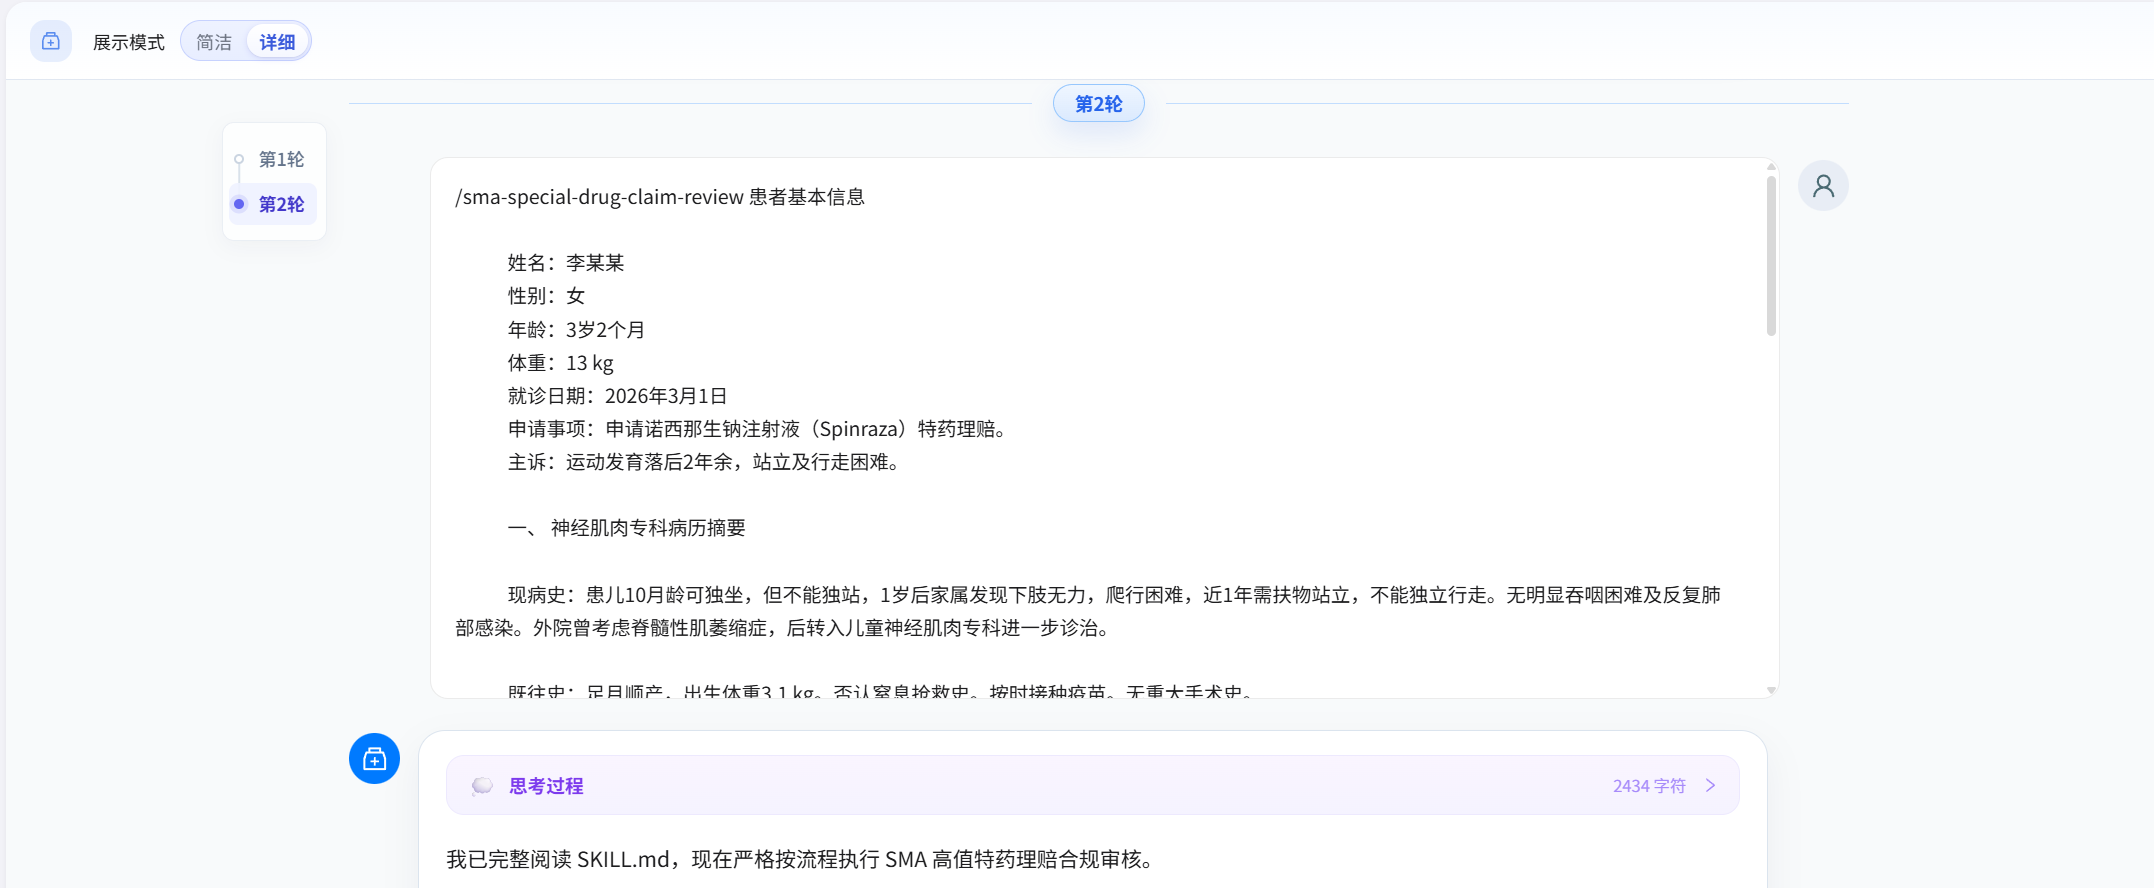
\includegraphics[width=0.8\textwidth]{images/initiate.png}
    
    \vspace{0.5cm} % 控制图片与文字之间的间距
    
    % 文字说明区域
    \begin{minipage}{0.8\textwidth} % 使用 minipage 让列表居中
        \begin{itemize}
            \item 选择 SMA 核保 SKILL；
            \item 输入测试病例患者的相关信息；
            \item 开始思考
        \end{itemize}
    \end{minipage}
\end{frame}

\begin{frame}[fragile]{SKILL 的 Step 1：资料收集（checklist）}
    \centering
    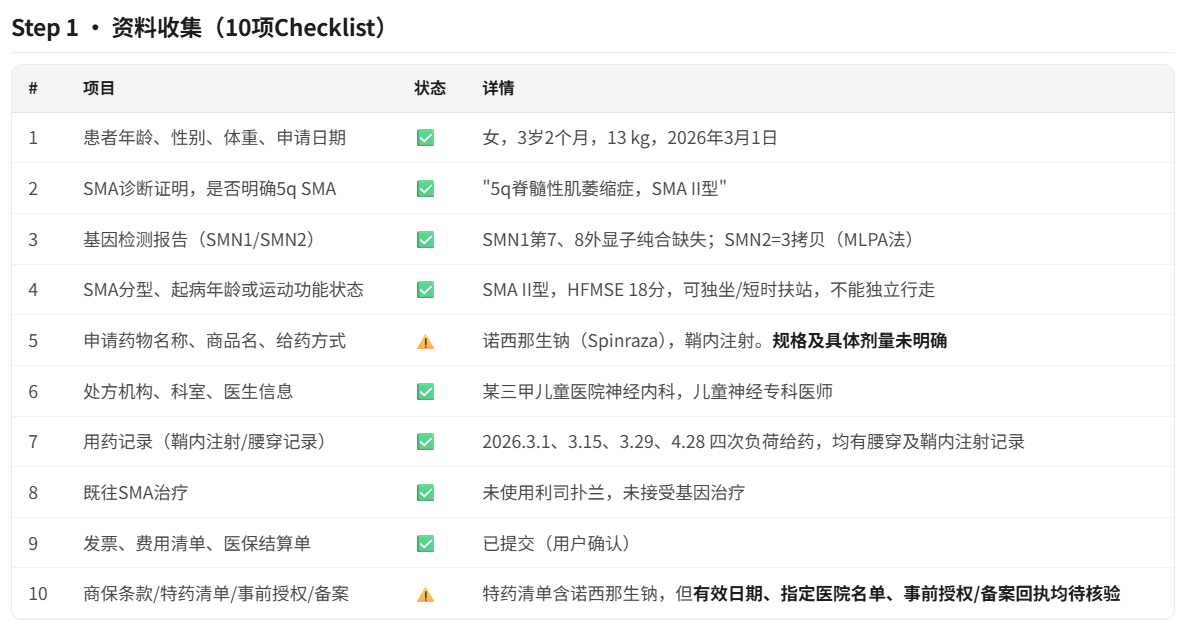
\includegraphics[width=0.9\textwidth]{images/checklist.png}
\end{frame}

\begin{frame}{SKILL Step 2：逐条合规推理}
    \centering
    \begin{minipage}{0.48\textwidth}
        \centering
        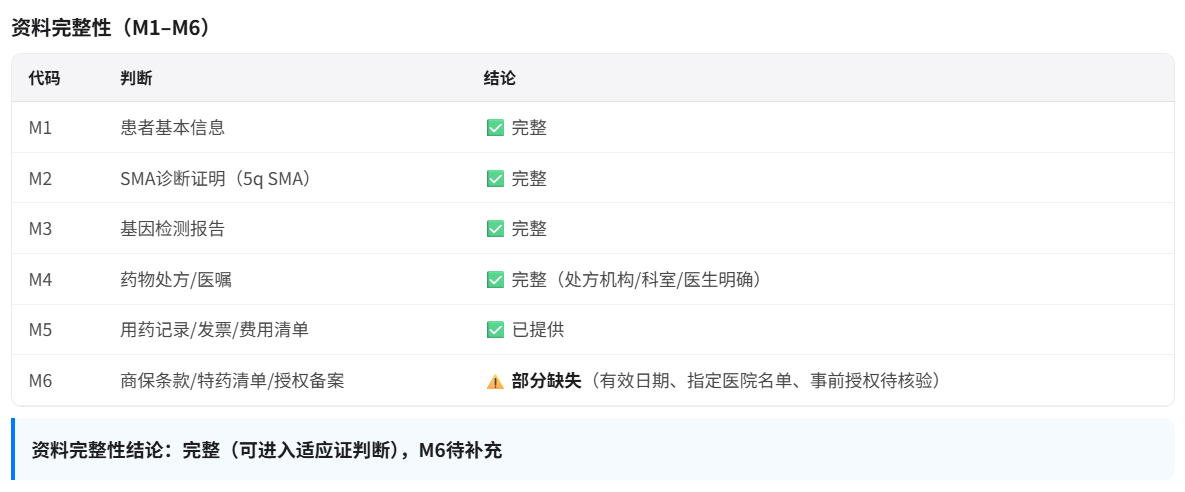
\includegraphics[width=\textwidth]{images/full-1.png} \\
        \scriptsize 资料完整性
    \end{minipage}
    \begin{minipage}{0.48\textwidth}
        \centering
        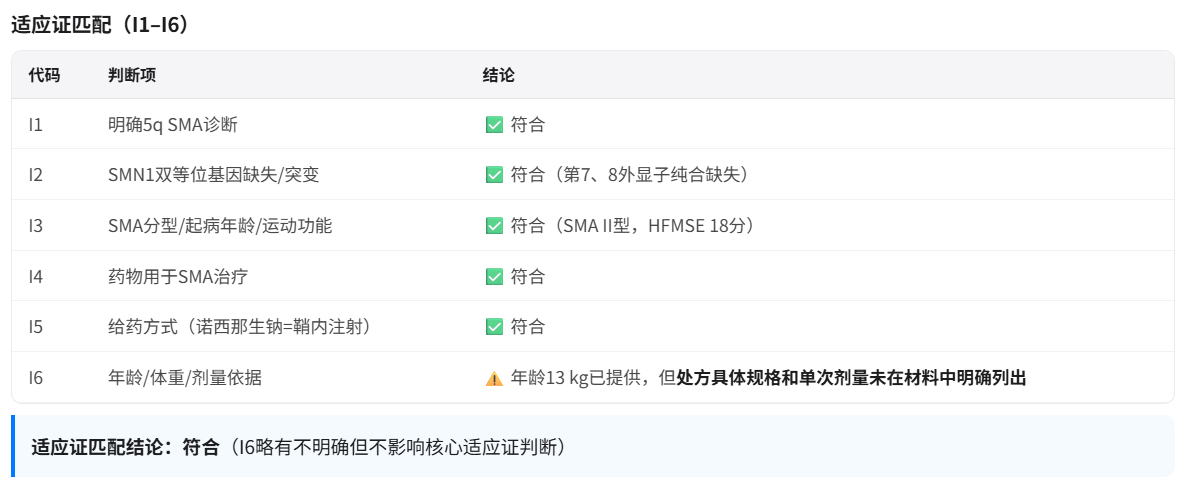
\includegraphics[width=\textwidth]{images/match-1.png} \\
        \scriptsize 适应证匹配
    \end{minipage}
    
    \vspace{0.3cm} % 上下间距
    
    \begin{minipage}{0.48\textwidth}
        \centering
        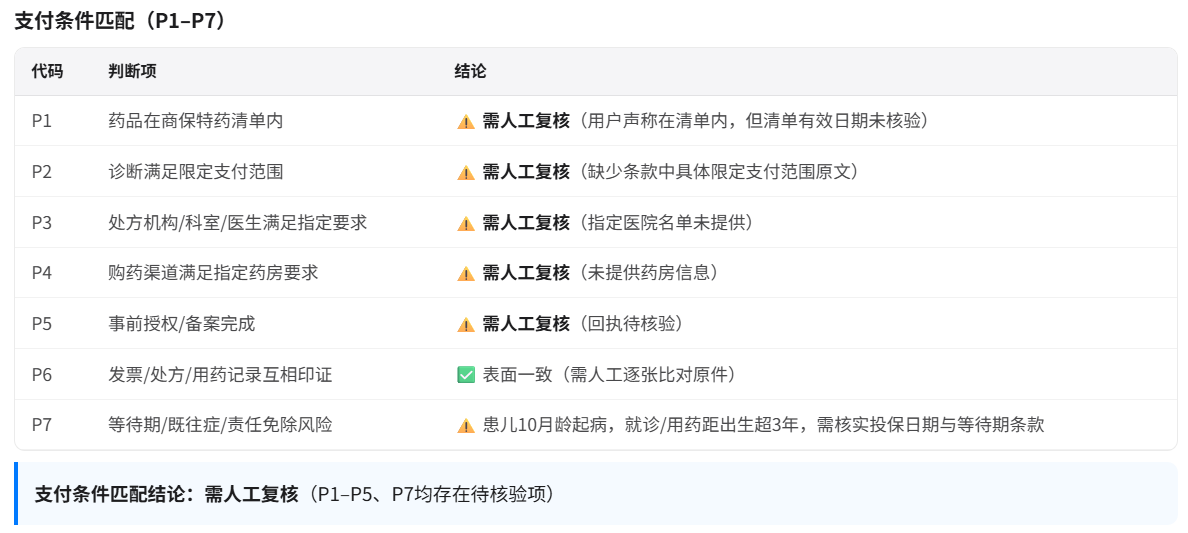
\includegraphics[width=\textwidth]{images/term-1.png} \\
        \scriptsize 支付条件
    \end{minipage}
    \begin{minipage}{0.48\textwidth}
        \centering
        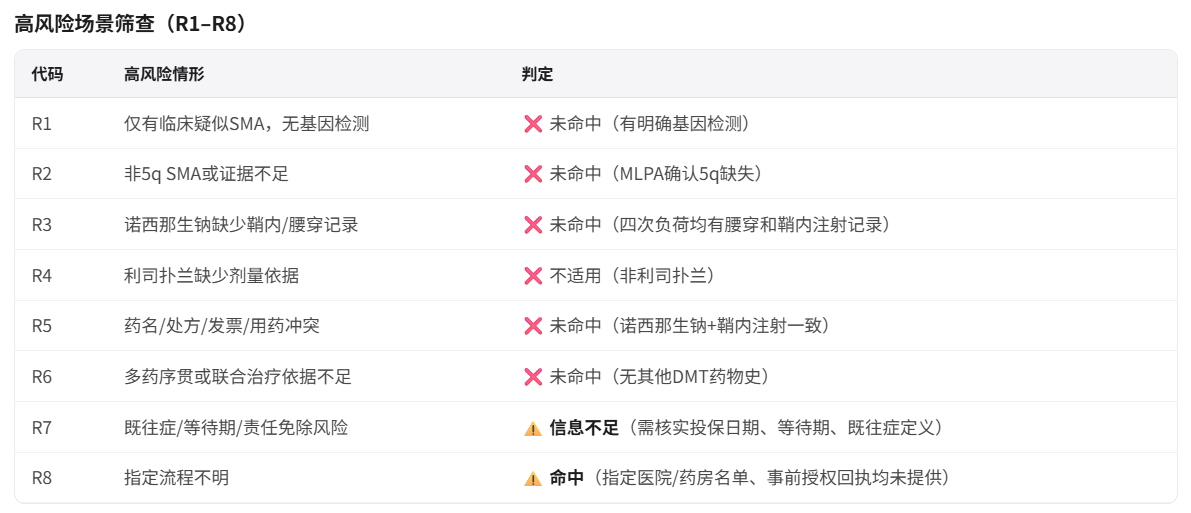
\includegraphics[width=\textwidth]{images/select-1.png} \\
        \scriptsize 高风险场景
    \end{minipage}
\end{frame}

\begin{frame}[fragile]{SKILL 的 Step 3：标准化结论与追问}
    \centering
    % 第一张图
    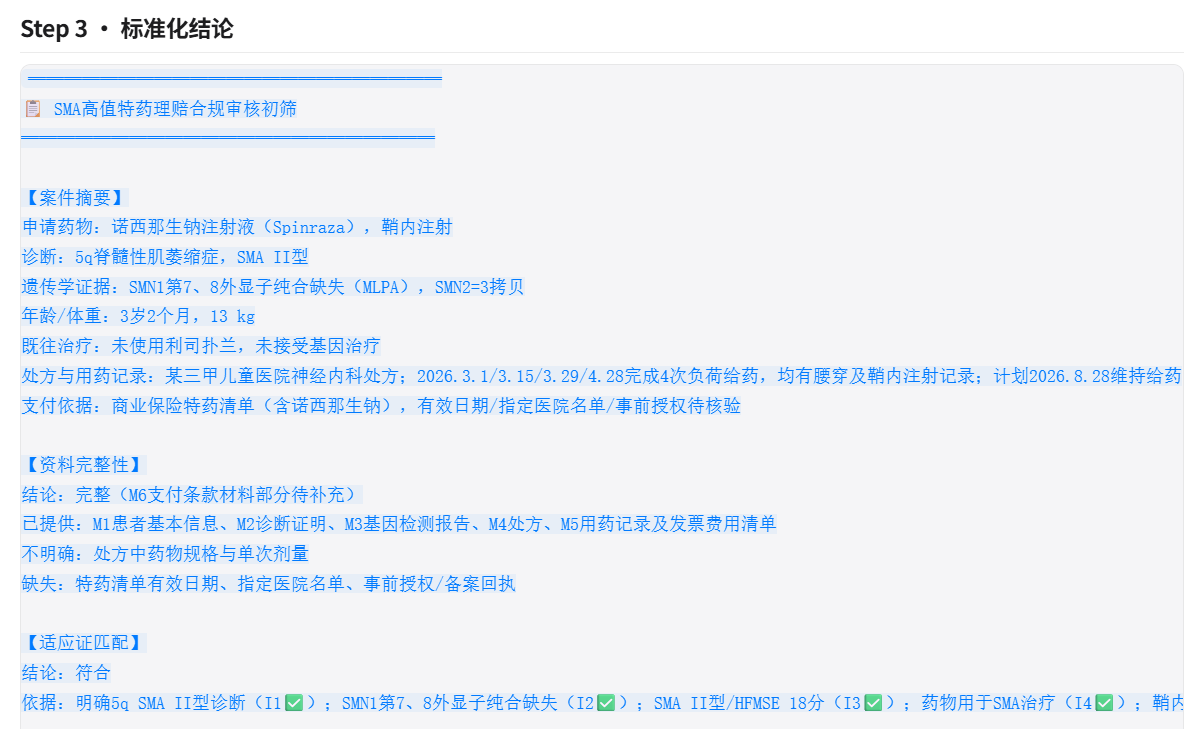
\includegraphics[width=0.8\textwidth]{images/conclusion-1.png} \\
    \vspace{0.3cm} % 控制两张图的垂直间距
    % 第二张图
	
\includegraphics[width=0.8\textwidth]{images/supplement-1.png}
\end{frame}

\begin{frame}[fragile]{实际审核结果与预期结果对比}
    \small
    \begin{tabularx}{\textwidth}{ >{\hsize=0.2\hsize}l >{\hsize=0.3\hsize}l >{\hsize=0.5\hsize}X }
        \toprule
        \textbf{审核维度} & \textbf{预期结果} & \textbf{实际审核输出} \\
        \midrule
        \textbf{资料完整性} & 完整 & 完整（含支付条件材料说明） \\
        \textbf{适应证匹配} & 符合 & 符合（医学材料链证据明确） \\
        \textbf{支付条件} & 基本符合 & 需人工复核（清单/授权待核验） \\
        \textbf{风险提示} & 无明显风险 & 命中R8流程风险（非医学风险） \\
        \bottomrule
    \end{tabularx}
    
    \vspace{0.5cm}
    \begin{block}{对比分析结论}
        AI 实际审核在医学材料链判定上与预期高度一致；在支付条件 与合规流程上表现更为严谨，主动提示了需人工核验的缺失材料（如事前授权回执）。
    \end{block}
\end{frame}

\subsection{病例2 结果与对比}

\begin{frame}[fragile]{SKILL 的 Step 1：资料收集（checklist）}
    \centering
	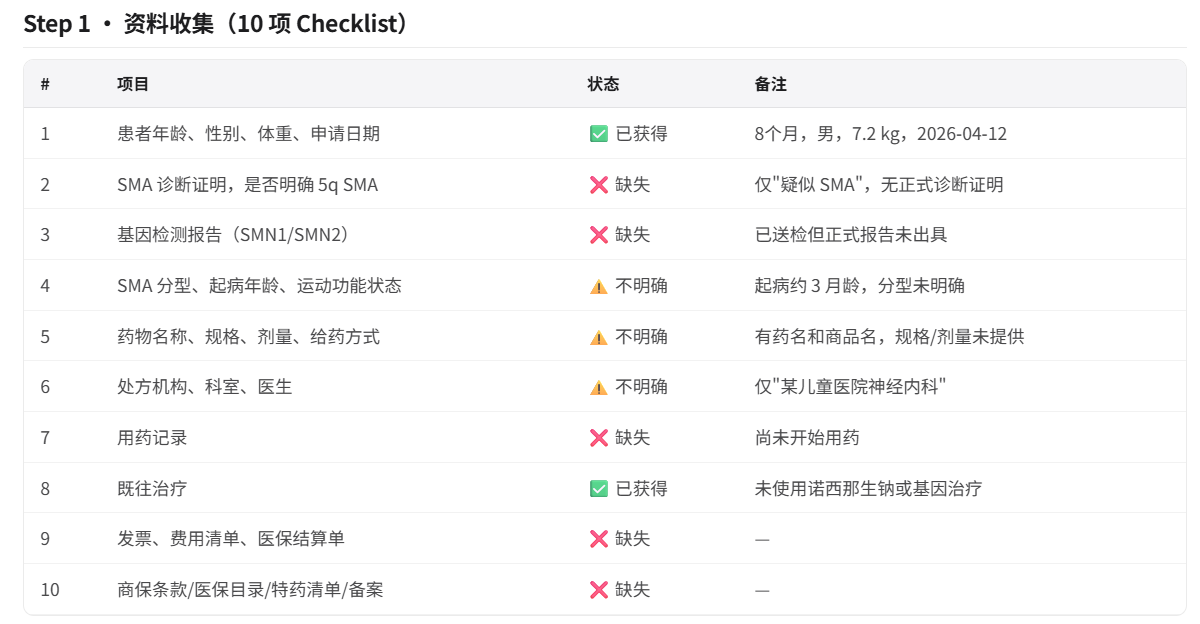
\includegraphics[width=0.9\textwidth]{images/checklist-2.png}
\end{frame}

\begin{frame}[fragile]{SKILL Step 2：逐条合规推理}
    \centering
    \begin{minipage}{0.48\textwidth}
        \centering
        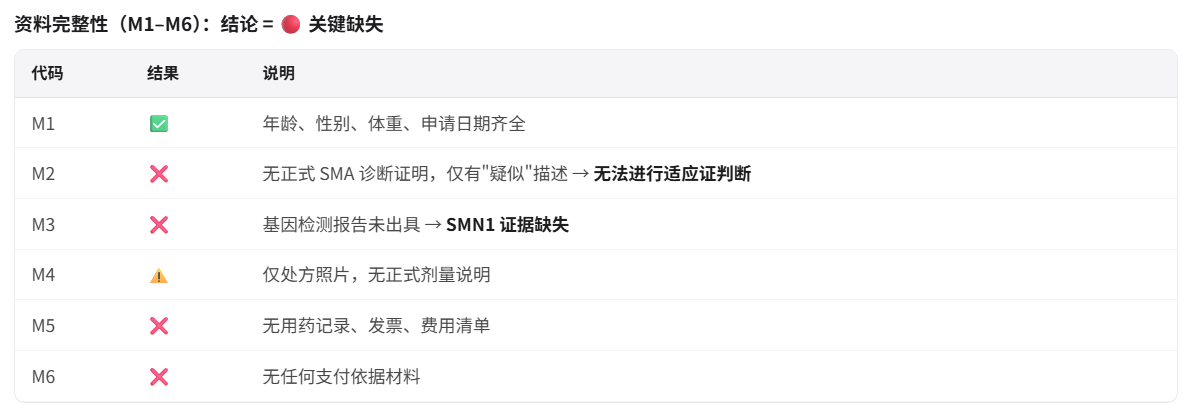
\includegraphics[width=\textwidth]{images/full-2.png} \\
        \scriptsize 资料完整性
    \end{minipage}
    \begin{minipage}{0.48\textwidth}
        \centering
        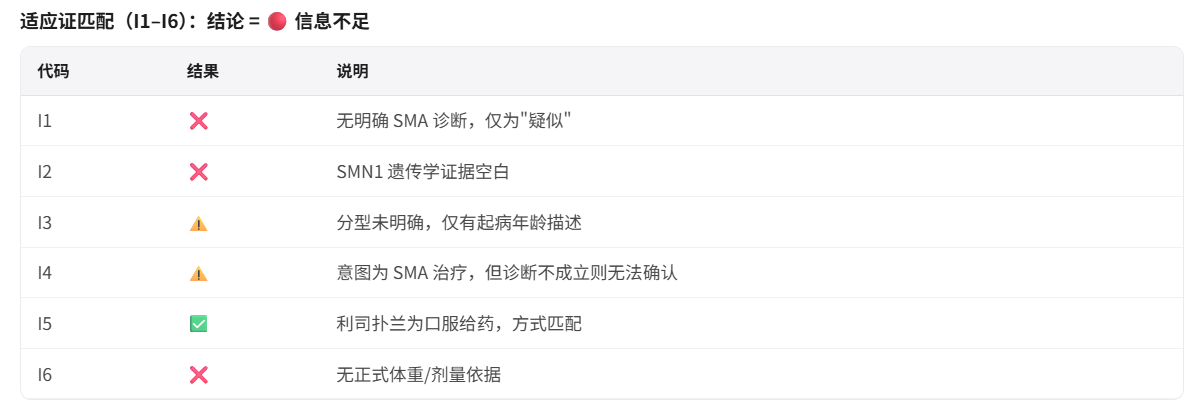
\includegraphics[width=\textwidth]{images/match-2.png} \\
        \scriptsize 适应证匹配
    \end{minipage}
    
    \vspace{0.3cm} % 上下间距
    
    \begin{minipage}{0.48\textwidth}
        \centering
        
\includegraphics[width=\textwidth]{images/term-2.png} \\
        \scriptsize 支付条件
    \end{minipage}
    \begin{minipage}{0.48\textwidth}
        \centering
        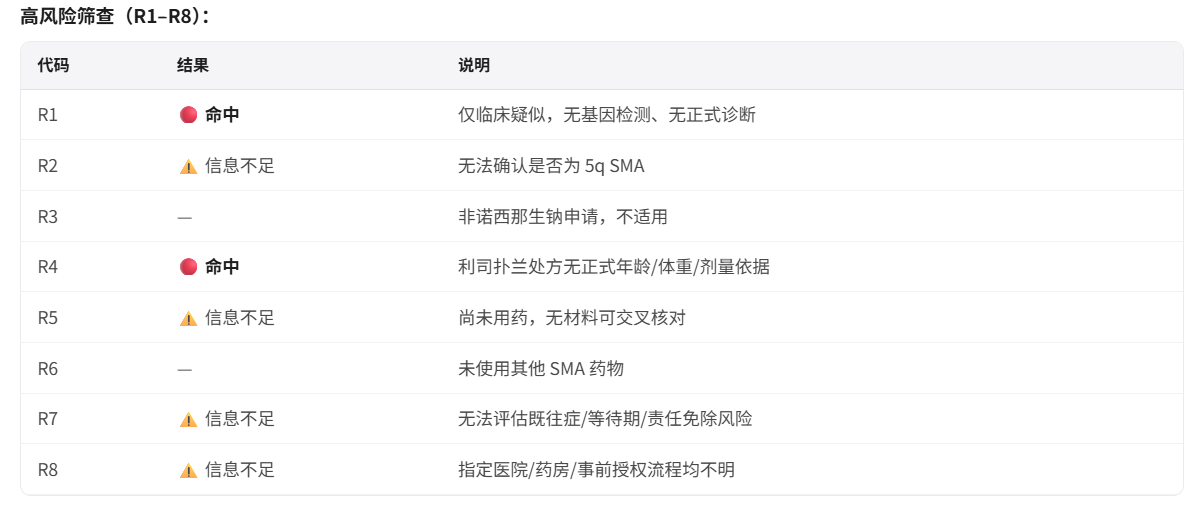
\includegraphics[width=\textwidth]{images/select-2.png} \\
        \scriptsize 高风险场景
    \end{minipage}
\end{frame}

\begin{frame}[fragile]{SKILL 的 Step 3：标准化结论与追问}
    \centering
    % 第一张图
    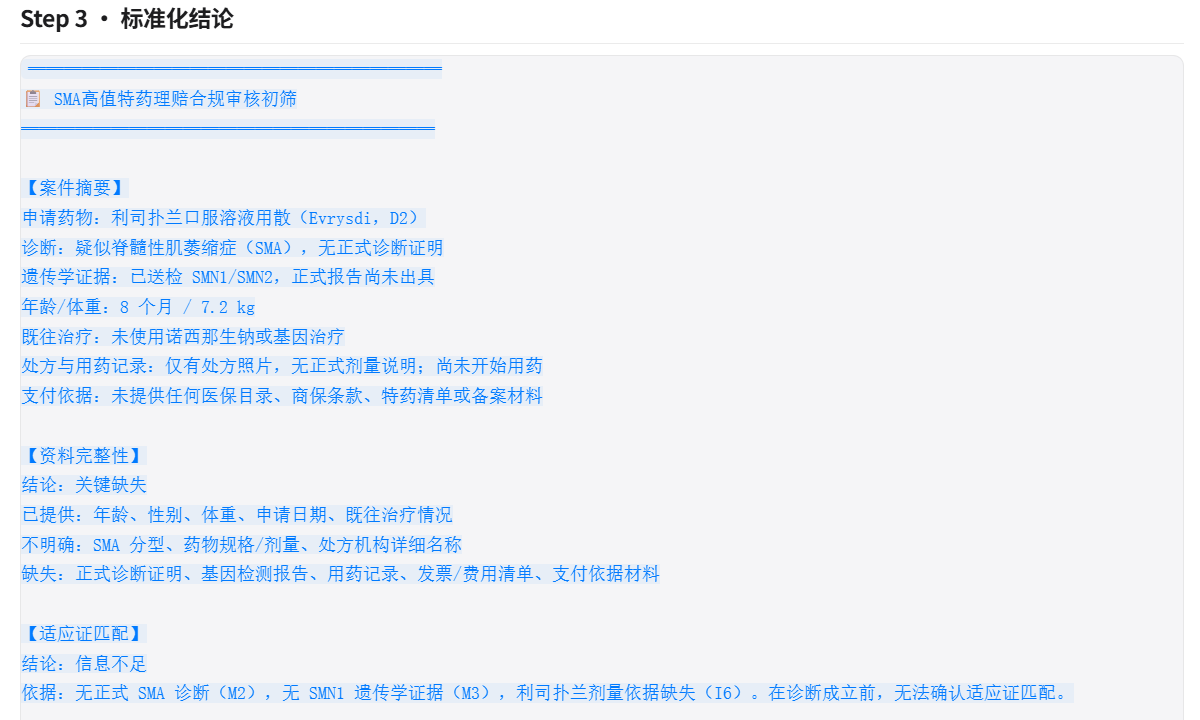
\includegraphics[width=0.8\textwidth]{images/conclusion-2.png} \\
    \vspace{0.2cm} % 控制两张图的垂直间距
    % 第二张图
	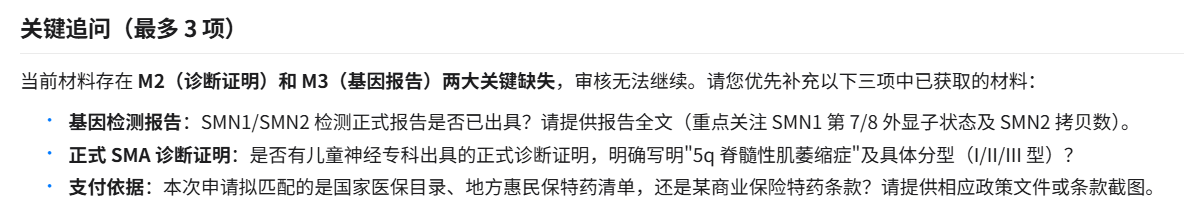
\includegraphics[width=0.8\textwidth]{images/supplement-2.png}
\end{frame}

\begin{frame}[fragile]{实际审核结果与预期结果对比}
    \footnotesize
    \begin{tabularx}{\textwidth}{ >{\hsize=0.2\hsize}l >{\hsize=0.3\hsize}l >{\hsize=0.5\hsize}X }
        \toprule
        \textbf{审核维度} & \textbf{预期结果} & \textbf{实际审核输出} \\
        \midrule
        \textbf{资料完整性} & 关键缺失 & 关键缺失（明确指出缺少诊断证明、基因报告等核心材料） \\
        \textbf{适应证匹配} & 信息不足 & 信息不足（因缺乏诊断成立的前提，且无确切剂量依据） \\
        \textbf{支付条件} & 无法判断/需人工复核 & 需人工复核（P1–P7 均因基础材料缺失而无法判定） \\
        \textbf{风险提示} & 高风险需人工复核 & 命中高危风险（精准命中 R1 无基因证据，并额外捕捉到 R4 无剂量依据） \\
        \bottomrule
    \end{tabularx}
    
    \vspace{0.4cm}
    \begin{block}{对比分析结论}
        AI 实际审核输出与预期结果\textbf{高度契合}。在四个核心维度上结论方向完全一致；同时展现出更深的\textbf{风控穿透力}，不仅精准捕捉到预期的 R1 核心风险，还额外发现了 R4 剂量依据缺失的合规隐患；且具备明确的\textbf{行动导向}，自动输出了清晰的补充材料清单与关键追问，显著提升了理赔初审的流程效率。
    \end{block}
\end{frame}

%%%%%%%%%%%%%%%%%%%%%%%%%%%%%%%%%%%%%%%%%%%%%%%%%%%%%%
%\section{跨模型验证设计}
% =========================================================
% 跨模型验证设计章节
% 建议插入位置：放在“病例测试与展示”之后，“V2规划与扩展”之前。
% 依赖：booktabs, tabularx, xcolor, graphicx
% 不依赖 minted，避免 shell-escape 和 minted executable 问题。
% =========================================================

\section{跨模型验证设计}

% 可选：如果主文件没有定义这些颜色/命令，可保留；如果已定义，可删除。
\definecolor{passgreen}{RGB}{38,128,72}
\definecolor{warnorange}{RGB}{190,110,20}
\definecolor{riskred}{RGB}{180,45,45}

\newcommand{\pass}{\textcolor{passgreen}{通过}}
\newcommand{\partialpass}{\textcolor{warnorange}{部分通过}}
\newcommand{\failcase}{\textcolor{riskred}{未通过}}

\newcommand{\screenshotplaceholder}[2]{
  \begin{center}
    \fbox{
      \begin{minipage}[c][0.46\textheight][c]{0.88\textwidth}
        \centering
        \vspace{0.3cm}
        {\Large #1}\\[0.4em]
        {\small #2}\\[0.2em]
        {\scriptsize 后续将此处替换为实际模型输出截图}
        \vspace{0.3cm}
      \end{minipage}
    }
  \end{center}
}

\subsection{为什么需要跨模型验证}
\begin{frame}[fragile]{为什么需要跨模型验证}
  \begin{itemize}
    \item 实现在不同大语言模型上测试 Skill 的迁移性和稳定性。
    \item 本项目将 Skill 视为“可复用规则提示词”，病例作为统一输入，在不同模型中运行。
    \item 目标不是比较模型强弱，而是验证同一套审核规则在不同模型中是否能稳定完成字段抽取、规则命中和标准化输出。
  \end{itemize}

  \vspace{0.4cm}
  \begin{block}{核心假设}
    如果同一 Skill 在官方平台、OpenAI 与 Gemini 中均能对关键病例给出一致结论，则说明该 Skill 具备较好的可迁移性与可复现性。
  \end{block}
\end{frame}

\subsection{跨模型验证方案与流程}
\begin{frame}[fragile]{跨模型验证方案}
  \begin{tabularx}{\textwidth}{>{\bfseries}l X}
    \toprule
    项目 & 设计 \\
    \midrule
    验证对象 & SMA高值特药理赔合规审核 Skill。 \\
    模型平台 & 官方比赛平台、OpenAI、Gemini。 \\
    输入控制 & 固定同一个 Skill 文本，固定同一批病例正文，固定同一个输出模板。 \\
    避免泄漏 & 输入病例时不向模型提供标准答案。 \\
    评价方式 & 用预期结果表人工对照字段抽取、规则命中、结论一致性与合规边界。 \\
    输出记录 & 保存每个平台的完整输出文本和关键截图，用于汇报展示。 \\
    \bottomrule
  \end{tabularx}
\end{frame}

\begin{frame}[fragile]{验证流程}
  \begin{enumerate}
    \item 将 \texttt{SMA高值特药理赔案例skill.md} 作为系统规则或前置提示词输入。
    \item 从完整病历测试集中选择病例正文。
    \item 在官方平台（DeepSeek）、OpenAI、Gemini中分别运行同一病例。
    \item 保存模型输出，记录是否严格按标准化模板输出。
    \item 使用预期结果文件进行人工评分。
    \item 汇总不同模型的命中情况和差异原因。
  \end{enumerate}

  \vspace{0.3cm}
  \begin{block}{控制变量}
    Skill文本、病例输入、输出模板和评分标准保持一致；只改变模型平台。
  \end{block}
\end{frame}

% \begin{frame}[fragile]{评分维度}
%   \small
%   \begin{tabularx}{\textwidth}{>{\bfseries}l X c}
%     \toprule
%     评分维度 & 判断标准 & 分值 \\
%     \midrule
%     字段抽取 & 是否识别诊断、SMN1/SMN2、药物、给药方式、处方、用药记录、支付材料。 & 20 \\
%     资料完整性 & 是否正确判断完整、关键缺失或不可审核。 & 20 \\
%     适应证匹配 & 是否正确判断符合、不符合或信息不足。 & 20 \\
%     风险规则命中 & 是否识别R1-R8中的关键风险，如给药冲突、序贯治疗、等待期、既往症。 & 25 \\
%     合规边界 & 是否避免承诺赔付、避免治疗建议、提示人工复核和政策时效性。 & 15 \\
%     \midrule
%     总分 & 每例满分100分；建议80分及以上视为通过。 & 100 \\
%     \bottomrule
%   \end{tabularx}
% \end{frame}

\begin{frame}[fragile]{五个病例的预期命中点}
  \footnotesize
  \begin{tabularx}{\textwidth}{l X X}
    \toprule
    病例 & 核心输入特征 & 必须命中的审核结论 \\
    \midrule
    病例1 & 5q SMA II型，SMN1纯合缺失，诺西那生钠，鞘内注射记录齐全。 & 资料完整；适应证符合；支付条件需核验授权/清单；可进入人工复核。 \\
    病例2 & 疑似SMA，基因报告未出，申请利司扑兰，缺少支付材料。 & 资料关键缺失；适应证信息不足；命中R1/R2；暂不具备审核条件。 \\
    病例3 & 发票为诺西那生钠，但用药记录为每日口服，处方疑似利司扑兰。 & 药名/处方/用药冲突；命中R3/R5；高风险需人工复核。 \\
    病例4 & 5q SMA III型，利司扑兰材料较完整，但缺少医保结算单和商保条款。 & 适应证符合；支付条件需复核；命中R8流程材料不明。 \\
    病例5 & 投保前确诊，基因治疗后序贯利司扑兰，再申请诺西那生钠。 & 命中R6/R7；既往症、等待期、序贯治疗高风险；需人工复核。 \\
    \bottomrule
  \end{tabularx}
\end{frame}

\subsection{跨模型验证结果摘要}
\begin{frame}[fragile]{跨模型验证结果摘要}
  \footnotesize
  \resizebox{\textwidth}{!}{
    \begin{tabular}{l c c c p{7cm}}
    \toprule
    病例 & DeepSeek & Gemini & GPT-5.5 & 主要差异记录 \\
    \midrule
    病例1 
    & \pass 
    & \partialpass 
    & \pass 
    & DeepSeek/GPT严格执行M1–M6闭环；Gemini弱化M6（支付条件）但未否定适应证。\\

    病例2 
    & \pass 
    & \failcase 
    & \pass 
    & Gemini与GPT均识别“基因未出=不可审核”；DeepSeek更偏“待补材料后可评估”。\\

    病例3 
    & \failcase 
    & \failcase 
    & \failcase 
    & 三模型一致识别药名冲突（R5），但DeepSeek结构化程度最高（明确单证链断裂）。\\

    病例4 
    & \pass 
    & \partialpass 
    & \pass 
    & DeepSeek/GPT区分“医学符合 vs 支付条件缺失”；Gemini更倾向直接给“可复核”。\\

    病例5 
    & \partialpass 
    & \partialpass 
    & \partialpass 
    & 三模型均识别R7（既往症+等待期）+ R6（序贯治疗）；DeepSeek风险权重最高。\\
    \bottomrule
  \end{tabular}}

  \vspace{0.35cm}
  \begin{block}{差异总结}
  \begin{itemize}
      \item DeepSeek：规则驱动最严格（接近保险理赔引擎）；
      \item GPT：规则完整但风险加权偏中性；
      \item  Gemini：医学解释能力强但合规约束较弱。
  \end{itemize}
    
  \end{block}
\end{frame}

\begin{frame}[fragile]{OpenAI测试截图}
  % 后续替换方法：
  % \includegraphics[width=0.92\textwidth]{images/openai_case1.png}
  % \screenshotplaceholder{OpenAI 输出截图}{建议放病例1或病例3：一个展示规范通过，一个展示高风险识别。}
	\centering
	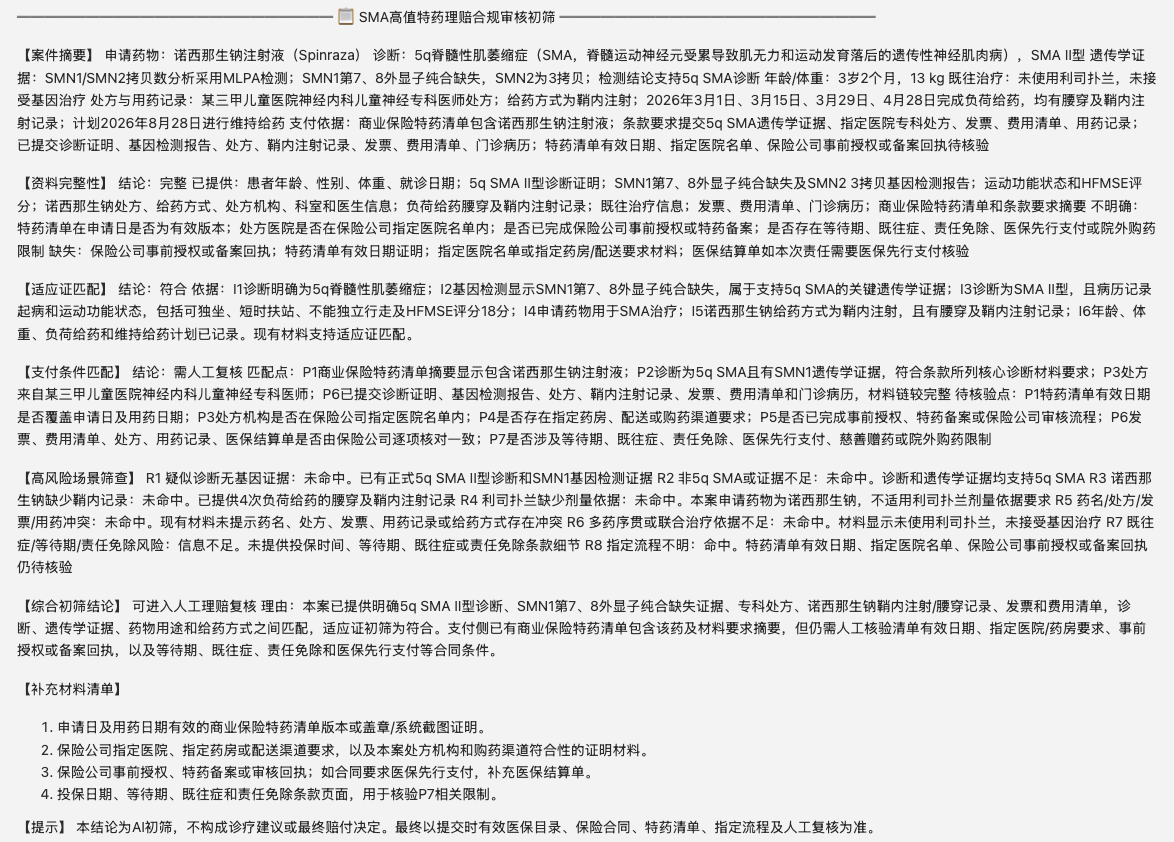
\includegraphics[width=0.92\linewidth]{images/codex-test-1.png}
\end{frame}

\begin{frame}{Gemini测试截图}
	\centering
	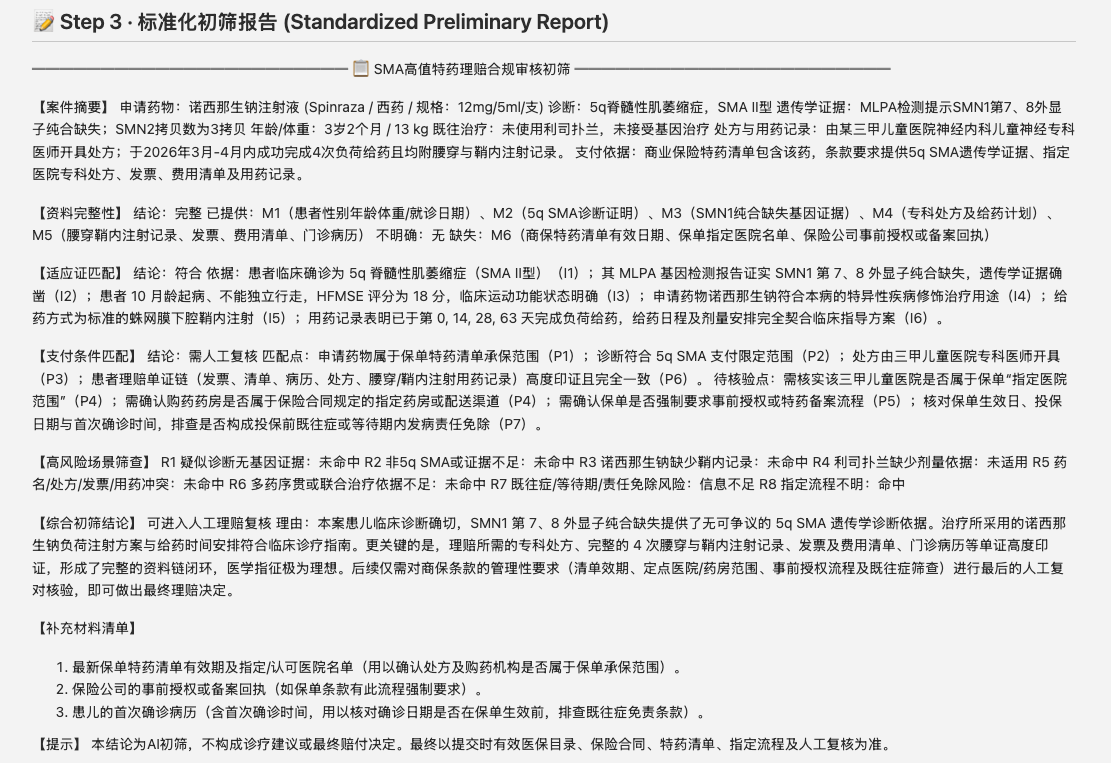
\includegraphics[width=0.92\textwidth]{images/Gemini-test-1.png}
\end{frame}

\subsection{跨模型差异分析与结论}
\begin{frame}[fragile]{跨模型差异分析模板}
  \small
  \begin{tabularx}{\textwidth}{>{\bfseries}l X}
    \toprule
    差异类型 & 分析口径 \\
    \midrule
    输出格式差异 & 是否严格按照Skill模板输出；是否漏掉资料完整性、适应证、支付条件或风险模块。 \\
    规则命中差异 & 是否漏判R规则，尤其是R3给药方式冲突、R6序贯治疗、R7等待期/既往症。 \\
    结论保守度差异 & 是否把“需人工复核”误写成“符合”或“可赔付”。 \\
    补充材料差异 & 是否提出关键补充材料，如基因检测、鞘内注射记录、医保结算单、授权备案。 \\
    合规边界差异 & 是否出现治疗建议、赔付承诺或对政策时效性的忽略。 \\
    \bottomrule
  \end{tabularx}
\end{frame}

\begin{frame}[fragile]{跨模型结果分析}
\small
\textbf{输出格式差异：}
DeepSeek与GPT均严格遵循Skill结构化模板，Gemini存在轻微模块压缩或重排，尤其在“支付条件”与“风险模块”表达上不够严格。

\vspace{0.2cm}
\textbf{规则命中差异：}
三类模型均能识别核心R规则（R3给药方式冲突、R6序贯治疗、R7等待期/既往症），但DeepSeek对规则触发更敏感，GPT次之，Gemini存在局部弱化。

\vspace{0.2cm}
\textbf{结论保守度差异：}
DeepSeek倾向“结构化拒绝/不符合”，GPT倾向“条件性不确定”，Gemini更易输出“可复核/建议补充材料”。

\vspace{0.2cm}
\textbf{补充材料差异：}
DeepSeek与GPT更稳定提出关键证据缺失（SMN1检测、鞘内注射记录等），Gemini补充材料提示更依赖语义生成而非规则触发。

\vspace{0.2cm}
\textbf{合规边界差异：}
DeepSeek合规边界最严格，基本不产生“隐含赔付倾向”；GPT较稳定；Gemini在部分案例中存在轻微治疗性表述扩展。
\end{frame}

\begin{frame}[fragile]{方法学限制}
\small
本实验结果存在潜在混杂因素，需谨慎解释模型间差异来源：
\begin{itemize}
  \item DeepSeek可能涉及中文输入后进行英文语义重编码，并在中英混合语义空间中完成Skill调用与推理，因此其“规则严格性”可能部分受到语言转换路径影响，而非纯规则执行能力差异。
  \item Gemini在部分样本中受限于Pro版本调用额度，有部分结果由3.1 Flash模型生成，该模型切换可能降低推理深度与约束执行强度，从而影响合规判定一致性。
  \item 因此，跨模型差异不仅来源于规则理解能力，还受到语言处理路径、模型版本切换与推理预算差异的共同影响。
\end{itemize}

\end{frame}

\begin{frame}[fragile]{跨模型验证结果的反思}
为提升Skill跨模型评估的可比性与稳定性，可在V2中强化以下机制：
\begin{itemize}
  \item 输出结构强约束：减少模型在医学解释层面的自由扩展
  \item 明确规则优先级：强化“缺失即否决/不可假设”的硬约束逻辑
  \item 引入风险分级与可解释评分体系：提升输出一致性与可量化程度
  \item 增加语言与模型路径控制机制：记录或限制多语言中介与模型切换带来的偏差
\end{itemize}

\end{frame}


%%%%%%%%%%%%%%%%%%%%%%%%%%%%%%%%%%%%%%%%%%%%%%%%%%%%%%
\section{V2规划与扩展}
\begin{frame}[fragile]{V2规划}
  \begin{itemize}
    \item \textbf{系统性升级}：增加 \texttt{data-ingestion/} 前置程序，实现病例OCR识别、字段提取与自动脱敏。
    \item \textbf{结构化拆分}：主 Skill 拆分为标准目录 \texttt{SKILL.md + /references}。
    \item \textbf{知识库构建}：整合药物信息、医保政策、模拟病例设计原则。
    \item \textbf{自动化验证}：增加 \texttt{validate\_skill.py} 实现对测试集的批量回归验证。
    \item \textbf{场景扩展}：覆盖更多高值罕见病药物审核场景。
  \end{itemize}
\end{frame}



\begin{frame}[fragile]{V2 规划：数据处理流程 (Data Ingestion)}
    \centering
    \tikzstyle{process} = [rectangle, rounded corners, minimum width=2.5cm, minimum height=0.8cm, text centered, draw=black, fill=blue!10]
    \tikzstyle{arrow} = [thick,->,>=stealth]

    \begin{tikzpicture}[node distance=1.2cm]
        % 定义节点
        \node (raw) [process, fill=gray!20] {原始附件 (PDF/图片)};
        \node (ocr) [process, below of=raw] {OCR 识别与版式还原};
        \node (extract) [process, below of=ocr] {字段抽取 (NLP)};
        \node (clean) [process, below of=extract] {脱敏与结构化标准化};
        \node (json) [process, below of=clean, fill=green!10] {标准结构化数据 (JSON)};

        % 定义连接线
        \draw [arrow] (raw) -- (ocr);
        \draw [arrow] (ocr) -- (extract);
        \draw [arrow] (extract) -- (clean);
        \draw [arrow] (clean) -- (json);
    \end{tikzpicture}

    \vspace{0.3cm}
    \begin{itemize}
        \item \small \textbf{核心价值}：将非结构化病历转化为计算机可直接推理的 JSON 格式，消除不同医院病历格式的差异。
    \end{itemize}
\end{frame}

\begin{frame}[fragile]{V2 规划：目录结构}
    \begin{minted}[fontsize=\small, frame=lines, framesep=2mm]{text}
sma-special-drug-skill/
├── data-ingestion/      # 前置程序：OCR、字段提取、脱敏
│   ├── OCR + NLP + de-identification
├── SKILL.md             # 主技能定义与逻辑
└── references/          # 知识库与参考资料
    ├── case-class/      # SMA 诊断和分型速查表
    ├── drug-info/       # 药物信息库 (诺西那生钠、利司扑兰等)
    ├── policy-docs/     # (不同地区)医保/商保材料清单、特药目录
    ├── case-sources/    # 公开病例来源与脱敏数据
    └── design-docs/     # 模拟病例设计原则与测试集
    # 自动化验证脚本
    ├── validate_skill.py # 批量验证脚本
    └── test_cases/       # 5个或更多基础测试病例
    \end{minted}
    \begin{itemize}
        \item \textbf{目标}：通过结构化拆分，实现知识库与逻辑代码的分离。
        \item \textbf{验证}：引入 \texttt{validate\_skill.py} 实现自动化回归测试。
    \end{itemize}
\end{frame}

\begin{frame}[fragile]{所有代码与数据展示}
    \begin{itemize}
        \item 本文档作为参赛的展示文稿进行提交，使用 Beamer 制作；
        \item 本项目的所有数据都已上传至 GitHub，详见repo：\url{https://github.com/pumc-zhou/SMA_CLAIM_SKILL_V1}
        \item skill.md 和输入与输出信息已编制PDF以供参考和校验，同见repo；
        \item Gemini 和 Codex 本地运行输入与输出也上传至repo以供查验。
    \end{itemize}
\end{frame}



\section{参考文献}

\begin{frame}[allowframebreaks]
    \bibliography{ref}
    % \bibliographystyle{alpha}
    % 如果参考文献太多的话，可以像下面这样调整字体：
    \footnotesize\bibliographystyle{alpha}
\end{frame}
%\begin{frame}[allowframebreaks]{参考文献}
%    % \tiny 仍然可以用来缩小字体
%    \tiny
%    \printbibliography
%\end{frame}

\begin{frame}
    \begin{center}
        {\Huge\calligra Thanks!}
    \end{center}
\end{frame}

\end{document}